\documentclass{article}
\usepackage{graphicx}

\begin{document}
\title{Requirements Specification Document}
\author{Team D}
\date{\today}

\maketitle

\vspace*{1.5in}
\begin{table}[htbp]
\caption{Team}
\begin{center}
\begin{tabular}{|r | c|}
\hline
Name & ID Number \\
\hline\hline
Stefanie Lavoie & 1951750 \\
Pinsonn Laverdure & 9684352 \\
Ghislain Ledoux & 6376320 \\
Rigil Malubay & 6262732 \\
Philippe Milot & 9164111 \\
Christopher Mukherjee & 6291929 \\
\hline
\end{tabular}
\end{center}
\end{table}

\pagenumbering{gobble}% Remove page numbers (and reset to 1)
\clearpage

\tableofcontents
\clearpage

\pagenumbering{arabic}% Arabic page numbers (and reset to 1)

\section{Introduction} % Status: To be done

This document will describe in detail the requirement specifications for the Vessel Monitoring System which is to be developed in the context of the COMP354 course. The requirements specifications include ... 

If a requirement appears in this document, the final Vessel Monitoring System \emph{must} conform to this requirement. Inversely, the Vessel Monitoring System is not required to conform to any other requirement that is not specified in this document.

\section{Architectural Design} % Status: To be done

[Detailed version of the architecture design pattern should be presented.
This section must give a high-level description of the system in terms of its modules and their respective purpose and exact interfaces.]

\subsection{Architecture Diagram}

The program as it is communicates in a completely different way that it previously does. Previously we had the main calling the information on a timer and sending them to the GUI which was making the program working all at the same time which was not what we wanted. The program now is separated into two subsystems; the VMS and simulator package working in parallel.

\begin{figure}[h]
\caption{Communication diagram of simulator package}
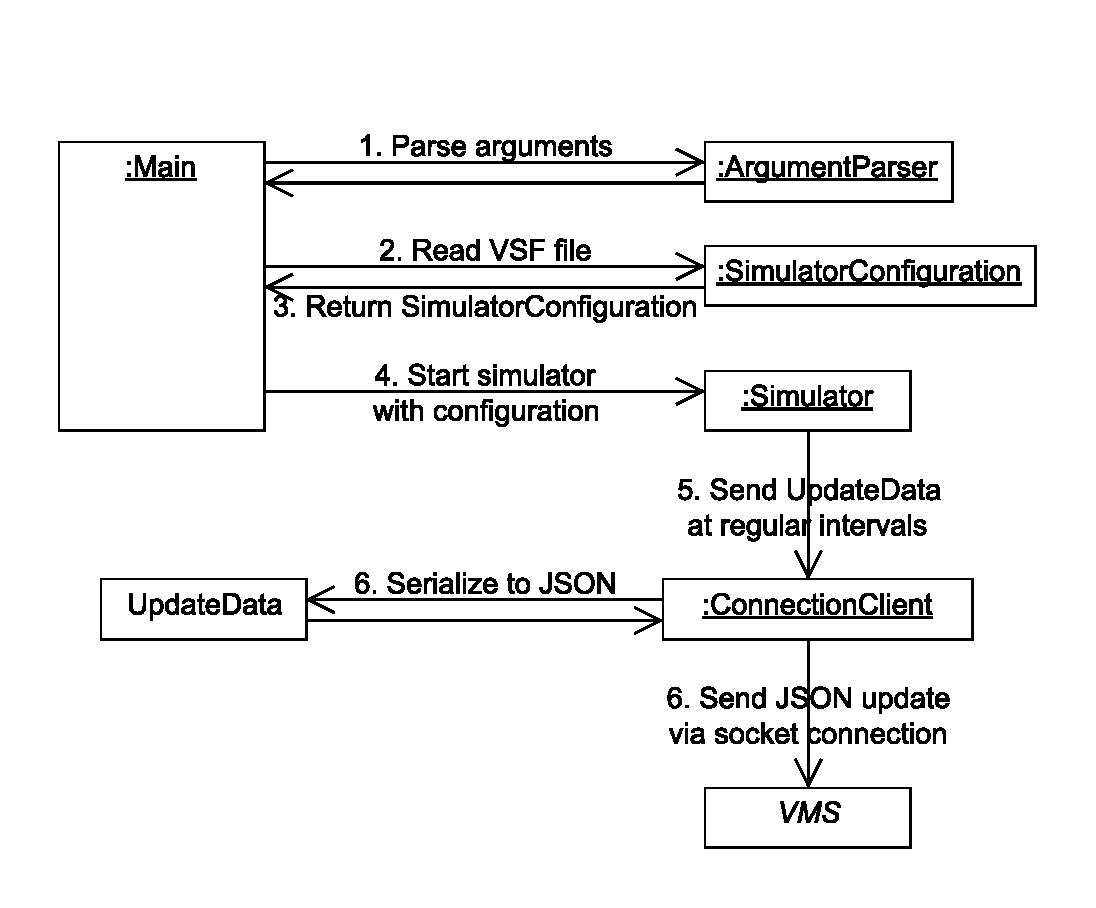
\includegraphics[width=\linewidth]{simulator-communication-diagram.eps}
\end{figure}

The simulator is in charge of making sure that the configuration is properly set into the sockets. Following the validation, the simulator will send the updated values at regular intervals to the VMS package.

\begin{figure}[h]
\caption{Communication diagram of vms package}
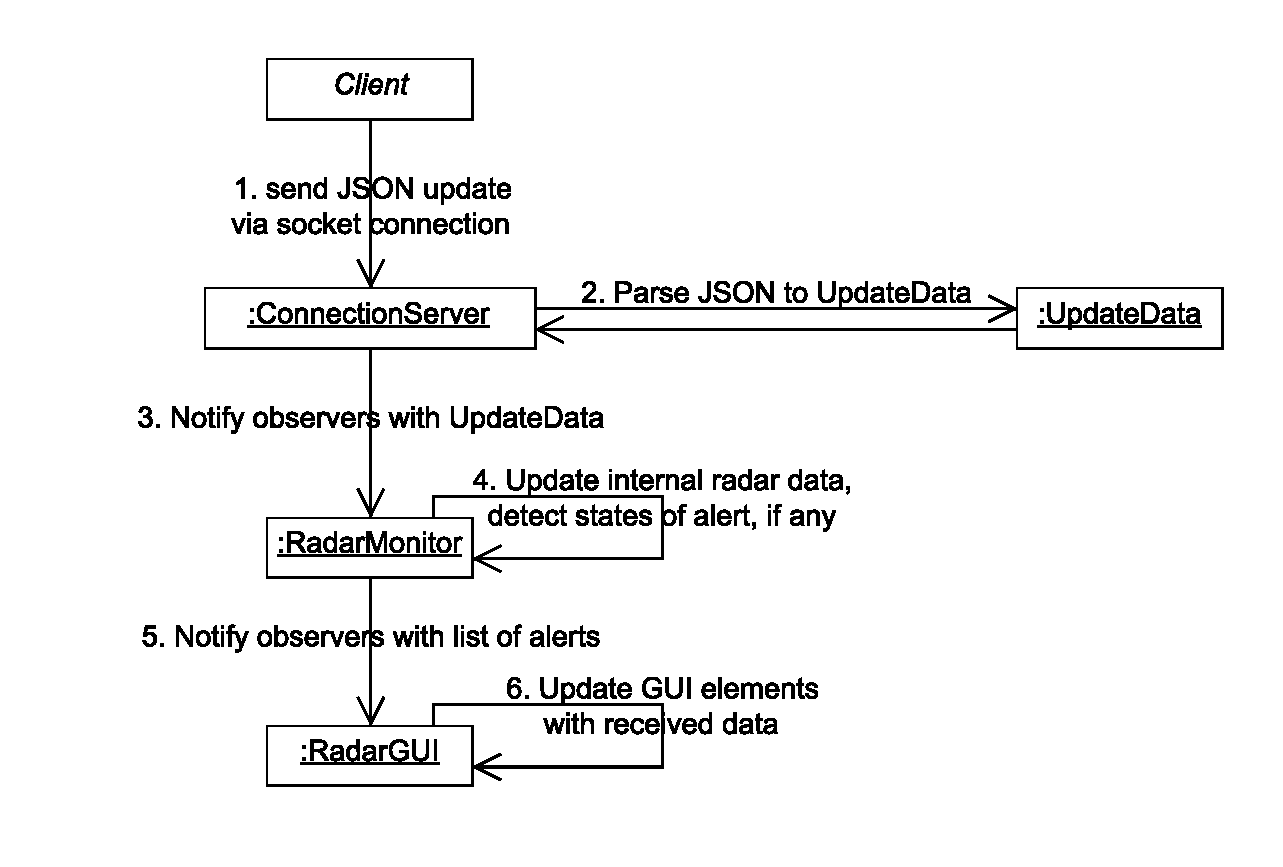
\includegraphics[width=\linewidth]{vms-communication-diagram.eps}
\end{figure}

The VMS package uses the observer pattern. The radar monitor and radar GUI are both observers of the server, so every time that the server is updated the monitor/GUI are also at the same time.

\subsection{Subsystem Interfaces Specifications}

[Specification of the software interfaces between the components, i.e. specific messages (or function calls) that are exchanged. These are also often called �Module Interface Specifications�.
Description of the parameters passed in these function calls in order to have a service fulfilled. Include valid and invalid ranges of values.
Each subsystem interface must be presented in a separate subsection.]

\break
\section{Detailed Design} % Status: To be done

\subsection{Subsystems} 

\subsubsection{Detailed Design Diagram}

[UML class diagram or equivalent depicting the internal structure of the subsystems, accompanied by a paragraph of text describing the rationale of the designs.]

\subsubsection{Unit Descriptions}

[List each class in the subsystem and write a short description of its purpose, as well as notes or reminders useful for the programmers who will implement them. List all attributes and functions of the class.]

\section{Dynamic Design Scenarios} % Status: To be done

[Give a full dynamic design of two substantial use cases including system sequence diagrams operational contracts, and sequence diagrams. Units and subsystems depicted here must be compatible with the descriptions provided in section 2 and 3.]

\section{Revised Cost Estimation} % Status: To be done

[Provide a revised estimated cost and schedule for the project, as well as the basis for those estimates, and the points and circumstances in the project when re-estimation might occur.
Evaluate the cost of production of each artifact, as described in the previous section, and then adding up the numbers.]

\emph{Software Design Document}: Three weeks of design and documentation. Due date: June 26th, 2013.

\emph{Simulator program}: Two weeks of coding, overlapped with SDD. Due date: June 26th, 2013.

\emph{Communication module}: Three weeks of coding, starting after the SDD is handed in. Due date: July 17th.

\emph{Alert computation module}: Two weeks of coding, starting after the SDD is handed in. Due date: July 10th.

\emph{Graphical User Interface}: Three weeks of coding, starting after the SDD is handed in. Due date: July 17th.

\emph{Unit test suite}: Six weeks of implementation, in parallel with SDD write-up and software implementation. Due date: July 17th.

\emph{Final integration}: Two weeks, after all other deliverables have been produced. Due date: July 31st.

\end{document}


